% Created by tikzDevice version 0.8.1 on 2016-02-05 23:23:45
% !TEX encoding = UTF-8 Unicode
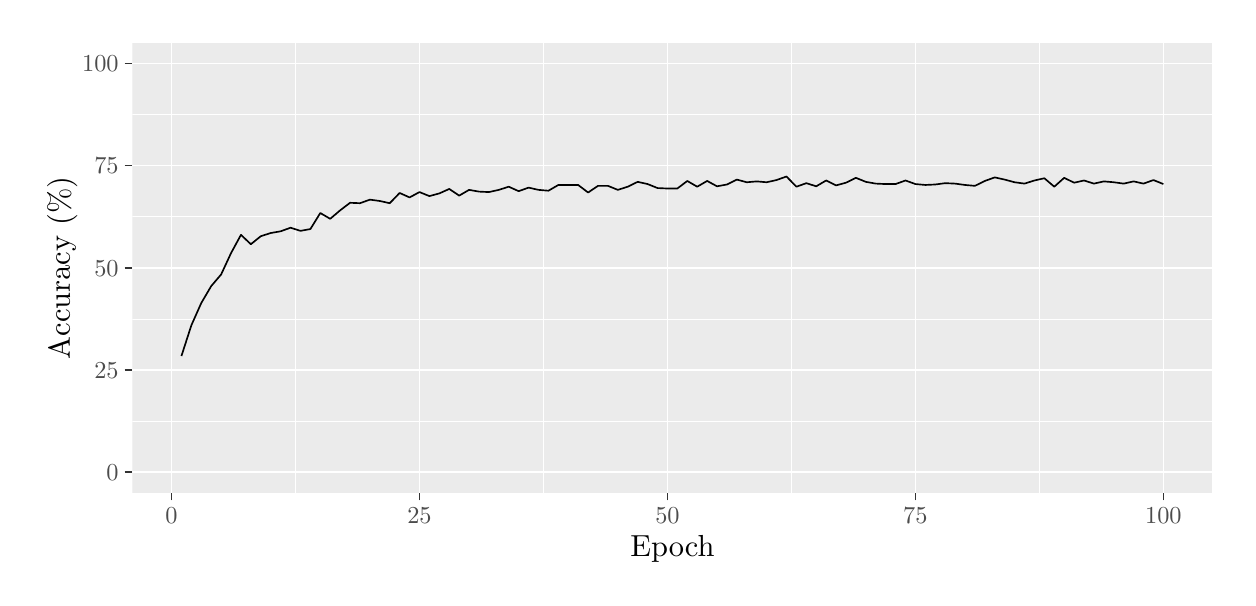
\begin{tikzpicture}[x=1pt,y=1pt]
\definecolor{fillColor}{RGB}{255,255,255}
\path[use as bounding box,fill=fillColor,fill opacity=0.00] (0,0) rectangle (433.62,198.74);
\begin{scope}
\path[clip] (  0.00,  0.00) rectangle (433.62,198.74);
\definecolor{drawColor}{RGB}{255,255,255}
\definecolor{fillColor}{RGB}{255,255,255}

\path[draw=drawColor,line width= 0.6pt,line join=round,line cap=round,fill=fillColor] (  0.00,  0.00) rectangle (433.62,198.74);
\end{scope}
\begin{scope}
\path[clip] ( 37.82, 30.69) rectangle (428.12,193.24);
\definecolor{fillColor}{gray}{0.92}

\path[fill=fillColor] ( 37.82, 30.69) rectangle (428.12,193.24);
\definecolor{drawColor}{RGB}{255,255,255}

\path[draw=drawColor,line width= 0.3pt,line join=round] ( 37.82, 56.55) --
	(428.12, 56.55);

\path[draw=drawColor,line width= 0.3pt,line join=round] ( 37.82, 93.49) --
	(428.12, 93.49);

\path[draw=drawColor,line width= 0.3pt,line join=round] ( 37.82,130.44) --
	(428.12,130.44);

\path[draw=drawColor,line width= 0.3pt,line join=round] ( 37.82,167.38) --
	(428.12,167.38);

\path[draw=drawColor,line width= 0.3pt,line join=round] ( 96.78, 30.69) --
	( 96.78,193.24);

\path[draw=drawColor,line width= 0.3pt,line join=round] (186.38, 30.69) --
	(186.38,193.24);

\path[draw=drawColor,line width= 0.3pt,line join=round] (275.98, 30.69) --
	(275.98,193.24);

\path[draw=drawColor,line width= 0.3pt,line join=round] (365.58, 30.69) --
	(365.58,193.24);

\path[draw=drawColor,line width= 0.6pt,line join=round] ( 37.82, 38.08) --
	(428.12, 38.08);

\path[draw=drawColor,line width= 0.6pt,line join=round] ( 37.82, 75.02) --
	(428.12, 75.02);

\path[draw=drawColor,line width= 0.6pt,line join=round] ( 37.82,111.96) --
	(428.12,111.96);

\path[draw=drawColor,line width= 0.6pt,line join=round] ( 37.82,148.91) --
	(428.12,148.91);

\path[draw=drawColor,line width= 0.6pt,line join=round] ( 37.82,185.85) --
	(428.12,185.85);

\path[draw=drawColor,line width= 0.6pt,line join=round] ( 51.98, 30.69) --
	( 51.98,193.24);

\path[draw=drawColor,line width= 0.6pt,line join=round] (141.58, 30.69) --
	(141.58,193.24);

\path[draw=drawColor,line width= 0.6pt,line join=round] (231.18, 30.69) --
	(231.18,193.24);

\path[draw=drawColor,line width= 0.6pt,line join=round] (320.78, 30.69) --
	(320.78,193.24);

\path[draw=drawColor,line width= 0.6pt,line join=round] (410.38, 30.69) --
	(410.38,193.24);
\definecolor{drawColor}{RGB}{0,0,0}

\path[draw=drawColor,line width= 0.6pt,line join=round] ( 55.56, 80.09) --
	( 59.15, 91.20) --
	( 62.73, 99.24) --
	( 66.32,105.36) --
	( 69.90,109.56) --
	( 73.48,117.27) --
	( 77.07,123.88) --
	( 80.65,120.49) --
	( 84.24,123.39) --
	( 87.82,124.53) --
	( 91.40,125.16) --
	( 94.99,126.45) --
	( 98.57,125.32) --
	(102.16,125.97) --
	(105.74,131.77) --
	(109.32,129.67) --
	(112.91,132.73) --
	(116.49,135.46) --
	(120.08,135.31) --
	(123.66,136.60) --
	(127.24,136.11) --
	(130.83,135.31) --
	(134.41,139.01) --
	(138.00,137.40) --
	(141.58,139.33) --
	(145.16,137.88) --
	(148.75,138.85) --
	(152.33,140.46) --
	(155.92,138.05) --
	(159.50,140.13) --
	(163.08,139.50) --
	(166.67,139.33) --
	(170.25,140.13) --
	(173.84,141.27) --
	(177.42,139.66) --
	(181.00,140.94) --
	(184.59,140.13) --
	(188.17,139.82) --
	(191.76,141.90) --
	(195.34,141.90) --
	(198.92,141.90) --
	(202.51,139.17) --
	(206.09,141.58) --
	(209.68,141.58) --
	(213.26,140.13) --
	(216.84,141.27) --
	(220.43,143.03) --
	(224.01,142.23) --
	(227.60,140.78) --
	(231.18,140.62) --
	(234.76,140.62) --
	(238.35,143.35) --
	(241.93,141.27) --
	(245.52,143.35) --
	(249.10,141.42) --
	(252.68,142.07) --
	(256.27,143.84) --
	(259.85,142.88) --
	(263.44,143.19) --
	(267.02,142.88) --
	(270.60,143.68) --
	(274.19,144.96) --
	(277.77,141.27) --
	(281.36,142.55) --
	(284.94,141.42) --
	(288.52,143.52) --
	(292.11,141.74) --
	(295.69,142.72) --
	(299.28,144.48) --
	(302.86,143.03) --
	(306.44,142.39) --
	(310.03,142.23) --
	(313.61,142.23) --
	(317.20,143.52) --
	(320.78,142.23) --
	(324.36,141.90) --
	(327.95,142.07) --
	(331.53,142.55) --
	(335.12,142.39) --
	(338.70,141.90) --
	(342.28,141.58) --
	(345.87,143.35) --
	(349.45,144.64) --
	(353.04,143.84) --
	(356.62,142.88) --
	(360.20,142.39) --
	(363.79,143.52) --
	(367.37,144.33) --
	(370.96,141.27) --
	(374.54,144.48) --
	(378.12,142.72) --
	(381.71,143.52) --
	(385.29,142.39) --
	(388.88,143.19) --
	(392.46,142.88) --
	(396.04,142.39) --
	(399.63,143.19) --
	(403.21,142.39) --
	(406.80,143.68) --
	(410.38,142.23);
\end{scope}
\begin{scope}
\path[clip] (  0.00,  0.00) rectangle (433.62,198.74);
\definecolor{drawColor}{gray}{0.30}

\node[text=drawColor,anchor=base east,inner sep=0pt, outer sep=0pt, scale=  0.88] at ( 32.87, 35.05) {0};

\node[text=drawColor,anchor=base east,inner sep=0pt, outer sep=0pt, scale=  0.88] at ( 32.87, 71.99) {25};

\node[text=drawColor,anchor=base east,inner sep=0pt, outer sep=0pt, scale=  0.88] at ( 32.87,108.93) {50};

\node[text=drawColor,anchor=base east,inner sep=0pt, outer sep=0pt, scale=  0.88] at ( 32.87,145.88) {75};

\node[text=drawColor,anchor=base east,inner sep=0pt, outer sep=0pt, scale=  0.88] at ( 32.87,182.82) {100};
\end{scope}
\begin{scope}
\path[clip] (  0.00,  0.00) rectangle (433.62,198.74);
\definecolor{drawColor}{gray}{0.20}

\path[draw=drawColor,line width= 0.6pt,line join=round] ( 35.07, 38.08) --
	( 37.82, 38.08);

\path[draw=drawColor,line width= 0.6pt,line join=round] ( 35.07, 75.02) --
	( 37.82, 75.02);

\path[draw=drawColor,line width= 0.6pt,line join=round] ( 35.07,111.96) --
	( 37.82,111.96);

\path[draw=drawColor,line width= 0.6pt,line join=round] ( 35.07,148.91) --
	( 37.82,148.91);

\path[draw=drawColor,line width= 0.6pt,line join=round] ( 35.07,185.85) --
	( 37.82,185.85);
\end{scope}
\begin{scope}
\path[clip] (  0.00,  0.00) rectangle (433.62,198.74);
\definecolor{drawColor}{gray}{0.20}

\path[draw=drawColor,line width= 0.6pt,line join=round] ( 51.98, 27.94) --
	( 51.98, 30.69);

\path[draw=drawColor,line width= 0.6pt,line join=round] (141.58, 27.94) --
	(141.58, 30.69);

\path[draw=drawColor,line width= 0.6pt,line join=round] (231.18, 27.94) --
	(231.18, 30.69);

\path[draw=drawColor,line width= 0.6pt,line join=round] (320.78, 27.94) --
	(320.78, 30.69);

\path[draw=drawColor,line width= 0.6pt,line join=round] (410.38, 27.94) --
	(410.38, 30.69);
\end{scope}
\begin{scope}
\path[clip] (  0.00,  0.00) rectangle (433.62,198.74);
\definecolor{drawColor}{gray}{0.30}

\node[text=drawColor,anchor=base,inner sep=0pt, outer sep=0pt, scale=  0.88] at ( 51.98, 19.68) {0};

\node[text=drawColor,anchor=base,inner sep=0pt, outer sep=0pt, scale=  0.88] at (141.58, 19.68) {25};

\node[text=drawColor,anchor=base,inner sep=0pt, outer sep=0pt, scale=  0.88] at (231.18, 19.68) {50};

\node[text=drawColor,anchor=base,inner sep=0pt, outer sep=0pt, scale=  0.88] at (320.78, 19.68) {75};

\node[text=drawColor,anchor=base,inner sep=0pt, outer sep=0pt, scale=  0.88] at (410.38, 19.68) {100};
\end{scope}
\begin{scope}
\path[clip] (  0.00,  0.00) rectangle (433.62,198.74);
\definecolor{drawColor}{RGB}{0,0,0}

\node[text=drawColor,anchor=base,inner sep=0pt, outer sep=0pt, scale=  1.10] at (232.97,  7.70) {Epoch};
\end{scope}
\begin{scope}
\path[clip] (  0.00,  0.00) rectangle (433.62,198.74);
\definecolor{drawColor}{RGB}{0,0,0}

\node[text=drawColor,rotate= 90.00,anchor=base,inner sep=0pt, outer sep=0pt, scale=  1.10] at ( 15.28,111.96) {Accuracy (\%)};
\end{scope}
\end{tikzpicture}
